% Effect of the splitting protocol on the accuracy of leaf-blade representations (slope chart).
% Build:  python make_fig_robust_leak_data.py
%         pdflatex fig_leak.tex && pdftoppm -png -r 600 -singlefile fig_leak.pdf fig_leak
\documentclass[border=3pt]{standalone}
\usepackage[T1]{fontenc}
\usepackage[scaled=0.92]{helvet}
\renewcommand{\familydefault}{\sfdefault}
\usepackage{sansmath}
\sansmath
\usepackage{pgfplots}
\pgfplotsset{compat=1.18}

\pgfplotsset{
  every axis/.append style={font=\small,line width=0.6pt,tick style={line width=0.6pt,black},
    axis line style={black},label style={font=\small},tick label style={font=\small}},
  leakA/.style={black!45,line width=1.0pt,mark=square*,mark size=2.1pt},
  leakB/.style={black!45,line width=1.0pt,dashed,mark=triangle*,mark size=2.6pt,mark options={solid}},
  leakC/.style={black!45,line width=1.0pt,dotted,mark=diamond*,mark size=2.6pt,mark options={solid}},
  leakD/.style={black!70,line width=1.0pt,dashdotted,mark=pentagon*,mark size=2.4pt,mark options={solid}},
  leakE/.style={black,line width=1.6pt,mark=*,mark size=2.6pt},
}

\begin{document}
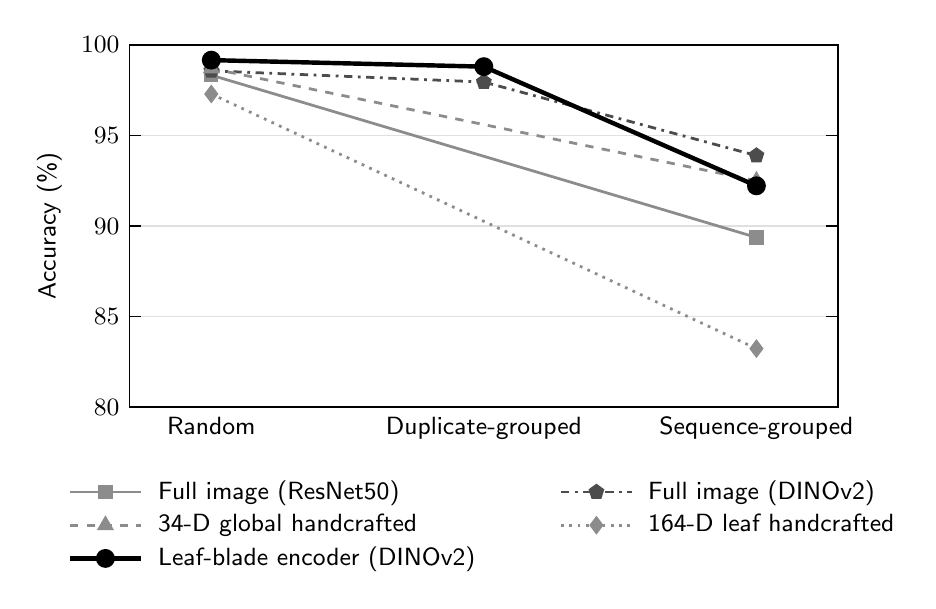
\begin{tikzpicture}
\begin{axis}[scale only axis,width=9.0cm,height=4.6cm,
    xmin=-0.3,xmax=2.3,xtick={0,1,2},xtick style={draw=none},
    xticklabels={Random,Duplicate-grouped,Sequence-grouped},
    ymin=80,ymax=100,ytick={80,85,...,100},ylabel={Accuracy (\%)},
    ymajorgrids,grid style={black!12,line width=0.4pt},
    % legend centred below the axis, two columns (full image | handcrafted | encoder)
    legend columns=2,
    legend style={draw=none,fill=none,font=\small,cells={anchor=west},
      /tikz/column 1/.style={column sep=0.12cm},/tikz/column 2/.style={column sep=1.0cm},
      /tikz/column 3/.style={column sep=0.12cm},
      at={(0.5,-0.17)},anchor=north},
    legend image code/.code={\draw[mark repeat=2,mark phase=2,#1] plot coordinates {(0cm,0cm) (0.45cm,0cm) (0.9cm,0cm)};}]
  % generated by make_fig_robust_leak_data.py
\addplot[leakA] coordinates {(0,98.33) (2,89.37)};
\addlegendentry{Full image (ResNet50)}
\addplot[leakD] coordinates {(0,98.57) (1,97.95) (2,93.89)};
\addlegendentry{Full image (DINOv2)}
\addplot[leakB] coordinates {(0,98.70) (2,92.50)};
\addlegendentry{34-D global handcrafted}
\addplot[leakC] coordinates {(0,97.29) (2,83.23)};
\addlegendentry{164-D leaf handcrafted}
\addplot[leakE] coordinates {(0,99.16) (1,98.80) (2,92.22)};
\addlegendentry{Leaf-blade encoder (DINOv2)}

\end{axis}
\end{tikzpicture}
\end{document}
